% This file was created with tikzplotlib v0.10.1.
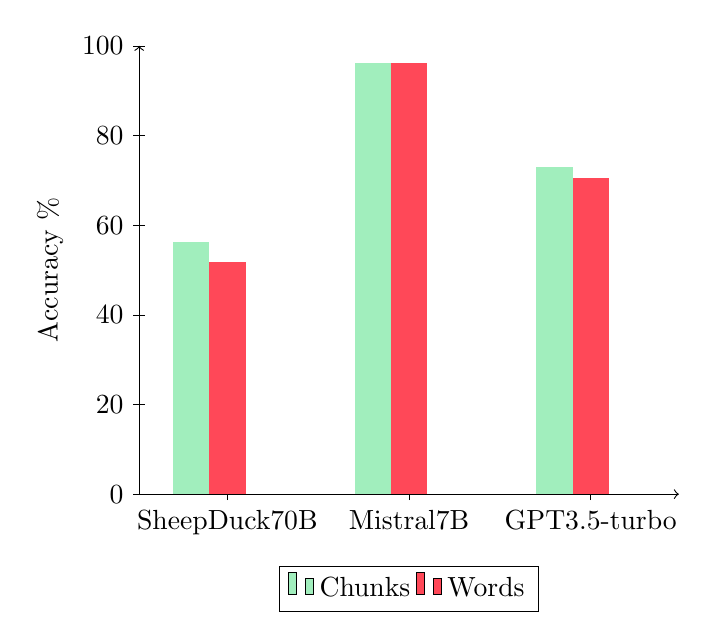
\begin{tikzpicture}

\definecolor{darkgray176}{RGB}{176,176,176}
\definecolor{limegreen018569}{HTML}{FF4858}
\definecolor{teal1293165}{HTML}{A1EEBD}

% \definecolor{xLightGreen}{HTML}{A1EEBD}
% \definecolor{xLightYellow}{HTML}{F6F7C4}
% \definecolor{xLightRed}{HTML}{F6D6D6}
% \definecolor{xLightBlue}{HTML}{7BD3EA}

\begin{axis}[
tick pos=both,
%title={Accuracy of the three models},
x grid style={black},
%xlabel={Model},
legend style={
    at={(0.5, -0.16)}, % Positions the legend below the x-axis
    anchor=north,      % Anchors the legend at its north side (top)
    legend columns=-1  % The number of columns the legend has, -1 for auto
},
xmin=-0.485, xmax=2.485,
xtick style={color=black},
xtick={0,1,2},
xticklabels={SheepDuck70B,Mistral7B,GPT3.5-turbo},
y grid style={black},
ylabel={Accuracy \%},
ymin=0, ymax=100,
ytick style={color=black},
ytick={0,20,40,60,80,100},
axis lines=left, % This keeps only the left and bottom axis lines
axis line style={->}, % This adds an arrow to the end of the axes
axis y line*=left, % Specifies that the y axis line should be on the left side
axis x line*=bottom, % Specifies that the x axis line should be on the bottom side
]
\draw[draw=none,fill=teal1293165] (axis cs:-0.3,0) rectangle (axis cs:-0.1,56.3030698889615);
\addlegendimage{ybar,ybar legend,draw=none,fill=teal1293165}
\addlegendentry{Chunks}

\draw[draw=none,fill=teal1293165] (axis cs:0.7,0) rectangle (axis cs:0.9,96.1463096015676);
\draw[draw=none,fill=teal1293165] (axis cs:1.7,0) rectangle (axis cs:1.9,72.8608752449379);
\draw[draw=none,fill=limegreen018569] (axis cs:-0.1,0) rectangle (axis cs:0.1,51.6982364467668);
\addlegendimage{ybar,ybar legend,draw=none,fill=limegreen018569}
\addlegendentry{Words}

\draw[draw=none,fill=limegreen018569] (axis cs:0.9,0) rectangle (axis cs:1.1,96.1789679947747);
\draw[draw=none,fill=limegreen018569] (axis cs:1.9,0) rectangle (axis cs:2.1,70.4114957544089);
\end{axis}

\end{tikzpicture}
